\documentclass[11pt,oneside,openany]{article}

\usepackage{graphicx}
\usepackage{color}    % to define macros for colors
\usepackage{listings} % package to include source code

\author{Matteo Franchin}

\title{Multiphysics~simulations of magnetic~nanostructures}

%TYPESETTING:----------------------------------------------------------

% Reset page margins properly for doublesided pages

% No headings
\pagestyle{plain}

% 1.5 interline spacing --> corresponds to linespread 1.3
% 2.0 interline spacing --> corresponds to linespread 1.6
\linespread{1.3}

\setlength{\marginparwidth}{0mm}
\setlength{\marginparsep}{0mm}
\setlength{\oddsidemargin}{0.7in} % corresponds to 1 + 0.7 = 1.7 inches
\setlength{\evensidemargin}{0.7in} % corresponds to 1.7 inches
\setlength{\textwidth}{145mm}
\setlength{\textheight}{220mm}
\setlength{\voffset}{-20mm}
\raggedbottom

%----------------------------------------------------------------------
% Extra colors

\definecolor{lightgrey}{cmyk}{0.05,0.05,0.05,0}
\definecolor{gray}{rgb}{0.5,0.5,0.5}

%----------------------------------------------------------------------
% Style for code listings

\lstdefinestyle{defaultstyle}{}
\lstset{language=Python}
\lstset{basicstyle=\ttfamily\scriptsize}
\lstset{showstringspaces=false}
\lstset{keywordstyle=\color{blue}}
\lstset{stringstyle=\color{red}}
\lstset{commentstyle=\color{gray}\emph}
\lstset{numbers=left,frame=single}
\lstset{backgroundcolor=\color{lightgrey}}

\begin{document}

\titlepage

\section{Applied field continuously varying in time with Nmag}
In this document we explain how to use Nmag to create a simulation where
the applied field changes continuously with time.
This is an undocumented feature, which can be used, but for which a clean
user interface has not been defined, yet.
Defining a field which changes continuously in time can be useful for many
purpose: applying a pulse with optimal time dependency to excite spin waves
inside a system (with a well controlled window of frequencies) or extending
Nmag by adding an extra term to the applied field.
In this document we will show and explain one example which was used
in the course of the DYNAMAG project to compute the susceptibility
of a disk (spin waves where excited for a defined window of frequencies).
In this example, it is important to apply an homogeneous (in space) magnetic
field with a time dependecy which goes as
$\mathrm{sinc} \, \omega_{\mathrm{max}} t$,
as this allows exciting spin waves with freqencies from 0 to
$\omega_{\mathrm{max}}$.

\subsection{The script}
\begin{figure}[t]
\begin{center}
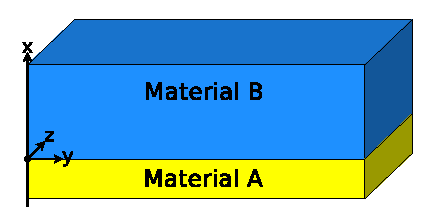
\includegraphics[width=10.0cm]{sketch}
\caption[Sketch]{A sketch of the system simulated in the script.}
\label{fig_es_types}
\end{center}
\end{figure}


\begin{figure}[!p]
\lstinputlisting[linerange=1-44]{script.py}
\caption{Part 1.}
\end{figure}

\begin{figure}[!p]
\lstinputlisting[linerange=45-92,firstnumber=45]{script.py}
\caption{Part 2.}
\end{figure}

\end{document}
